\documentclass[a4paper,12pt]{article} % тип документа
\usepackage[margin=1in]{geometry} % Поля

%  Русский язык
\usepackage[warn]{mathtext}
\usepackage[T2A]{fontenc}			% кодировка
\usepackage[utf8]{inputenc}			% кодировка исходного текста
\usepackage[english,russian]{babel}	% локализация и переносы
% Математика
\usepackage{amsmath,amsfonts,amssymb,amsthm,mathtools} 
\usepackage{wasysym}
%%%
\usepackage{graphicx}

\usepackage{tabularx}

\usepackage{minted} % код
%\usepackage{isotope} % изотоп

\usepackage{gensymb} % знак градуса
\usepackage{enumitem} % изменить список enumerate
\usepackage{placeins} % \FloatBarrier

\renewcommand{\thesection}{\Roman{section}} 
\renewcommand{\thesubsection}{\roman{subsection}}
\renewcommand{\thesubsubsection}{\roman{subsection}.\alph{subsubsection}}



\begin{document}

\newcolumntype{Y}{>{\centering\arraybackslash}X} %new tabularx


%титул
\hrule 	
\medskip
\begin{raggedright}
{\large \textbf{Отчёт по работе 5.5.5}}
\\
\medskip
{\Large Компьютерная сцинтилляционная гамма-спектрометрия} 
\\
\medskip
{\large Бичина Марина, Карташов Констанин Б04-005}
\medskip
\hrule
\medskip
\end{raggedright}


\section{Анотация}

\paragraph{Цель работы:} 
Измерение и определение энергий и интенсивности дискретных гамма-линий от различных гамма-источников и их идентификации.

\paragraph{Оборудование:}
\begin{itemize}
\renewcommand{\labelitemi}{$\triangleright$}
\itemsep0em
\item Гамма-источники: $^{22}_{11}$Na, $^{60}_{27}$Co, $^{137}_{55}$Cs, $^{152}_{63}$Eu, $^{241}_{95}$Am
\item Сцинтилляционный гамма-спектрометр (сцинтиллятор, ФЭУ, предусилитель)
\item АЦП для преобразования импульсов с ФЭУ
\item Компьютер для сбора данных, их обработки и хранения
\end{itemize}


\medskip\hrule\medskip

\section{Теоретическая часть}

\paragraph{}Основными процессами взаимодействия гамма-излучения с веществом являются фотоэффект, эффект Комптона и образование электрон-позитронных пар. Каждый из этих процессов вносит свой вклад в образование наблюдаемого спектра. Образующиеся при этих процессах электроны испытывают большое количество неупругих соударений с молекулами и атомами среды. Неупругие соударения могут сопровождаться как ионизацией, так и возбуждением молекул или атомов среды. В промежуточных же стадиях (при переходах возбуждённых молекул или атомов в основное состояние, при рекомбинации электрических зарядов и т.п.) в веществе возникают кванты света различных длин волн, присущих данному веществу.
	
При \textbf{фотоэффекте} кинетическая энергия электрона $ T_e = E_\gamma - I_i $, где $ I_i $ -- энергия ионизации $ i $-той оболочки атома. Фотоэффект особенно существенен для тяжёлых веществ, где он идёт с заметной вероятностью даже при высоких энергиях гамма-квантов. В лёгких веществах фотоэффект становится заметен лишь при относительно небольших энергиях гамма-квантов. Наряду с фотоэффектом, при котором вся энергия гамма-кванта передаётся атомному электрону, взаимодействие гамма-излучения со средой может приводить к его рассеянию, т.е. отклонению от первоначального направления распространения на некоторый угол.
	
При \textbf{эффекте Комптона} происходит упругое рассеяние фотона на свободном электроне, сопровождающееся изменением длины волны фотона (реально этот процесс происходит на слабо связанных с атомом внешних электронах). Максимальная энергия образующихся комптоновских электронов соответствует рассеянию гамма-квантов на $ 2\pi $ и равна:
	
	\begin{equation}
	E_{\max} = \dfrac{\hbar \omega}{1 + \dfrac{m_ec^2}{2\hbar\omega}}.
	\label{e:compton}
	\end{equation}
	
При достаточно высокой энергии гамма-кванта наряду с фотоэффектом и эффектом Комптона может происходить третий вид взаимодействия гамма-квантов с веществом – \textbf{образование электрон-позитронных пар}. При этом если процесс образования пары идет в кулоновском поле ядра или протона, то энергия образующегося ядра отдачи оказывается весьма малой, так что пороговая энергия гамма-кванта, необходимая для образования пары, практически совпадает с удвоенной энергией покоя электрона $Е_0 = 2m_ec^2 =1,022$ МэВ.
	
Появившийся в результате процесса образования пар электрон теряет свою энергию на ионизацию среды. Таким образом, вся энергия электрона остаётся в детекторе. Позитрон будет двигаться до тех пор, пока практически не остановится, а затем аннигилирует с электроном среды, в результате чего появятся два гамма-кванта. Т.е., кинетическая энергия позитрона также останется в детекторе. Далее возможны три варианта развития событий:
	
	а) оба родившихся гамма-кванта не вылетают из детектора, и тогда вся энергия первичного гамма-кванта останется в детекторе, а в спектре появится пик с $E = E_\gamma$;
	
	б) один из родившихся гамма-квантов покидает детектор, и в спектре появляется пик, соответствующий энергии $ Е = Е_\gamma - E_0$, где $ Е_0 = m_ec^2 = $ 511 кэВ;
	
	в) оба родившихся гамма-кванта покидают детектор, и в спектре появляется пик, соответствующий энергии $Е = Е_\gamma - 2E0$, где $2Е_0 = 2m_ec^2 = $ 1022 кэВ;
	
Таким образом, любой спектр, получаемый с помощью гамма-спектрометра, описывается несколькими компонентами, каждая из которых связана с определённым физическим процессом. Как описано выше, основными физическими процессами взаимодействия гамма-квантов с веществом являются фотоэффект, эффект Комптона и образование электрон-позитронных пар, и каждый из них вносит свой вклад в образование спектра. Помимо этих процессов, добавляются экспонента, связанная с наличием фона, пик характеристического излучения, возникающий при взаимодействии гамма-квантов с окружающим веществом, а также пик обратного рассеяния, образующийся при энергии квантов $ Е_\gamma \gg mc^2 $ в результате рассеяния гамма-квантов на большие углы на материалах конструктивных элементов детектора и защиты. Положение пика обратного рассеяния определяется по формуле ($ E $ -- энергия фотопика):
	
	\begin{equation}
		E_{обр} = \dfrac{E}{1 + \dfrac{2E}{mc^2}}.
		\label{e:compron_back}
	\end{equation}

	
Энергетическим разрешением спектрометра называется величина:
	
	\begin{equation}\label{e:resolution}
	R_i = \dfrac{\Delta E_i}{E_i},
	\end{equation}
	
\noindent т.е. отношение ширины пика полного поглощения (измеренной на полу-высоте) к регистрируемой энергии пика поглощения. Это значение $ E_i \propto \overline{n_i} $ --- числу частиц на выходе ФЭУ. При этом  $ \Delta E_i \propto \overline{\Delta n_i} = \sqrt{\overline{n_i}} $ --- ширина пика пропорциональна среднеквадратичной флуктуации, которая равна корню из числа частиц. Таким образом, наша формула \eqref{e:resolution} примет вид:
	
	\begin{equation}\label{e:res_law}
	R_i = \dfrac{\mathrm{const}}{\sqrt{E_i}}
	\end{equation}

\medskip\hrule\medskip

\section{Экспериментальная часть}

\subsection{Проведение измерений и подготовка данных к обработке}

\paragraph{}При помощи гамма-спектрометра измерим спектры для каждого образца и фонового излучения с временем воздействия $\sim 600$ с. Так как нам известно точное время воздействия нормализуем спектры относительно $600$ с, поделив полученные значения на $\tau / 600$, где $\tau$ -- действительное время воздействия. Это позволит нам сравнить интенсивности гамма-спектров для различных источников, а также вычесть фоновое излучение.

\paragraph{}Учтём фоновое излучение. Для этого вычтем из каждого спектра приближённое значение фонового излучения, если при этом получаться отрицательные значения, то заменим из на ноль. Измеренный спектр фонового излучения и приближённое значения показаны на рис. \ref{fig:bg}. Приближённое значения получено при помощи сглаживающего сплайна с параметром сглаживания $\lambda = 2400$ (\mintinline{python}|UnivariateSpline| из scipy).

\begin{figure}[h]
\centering
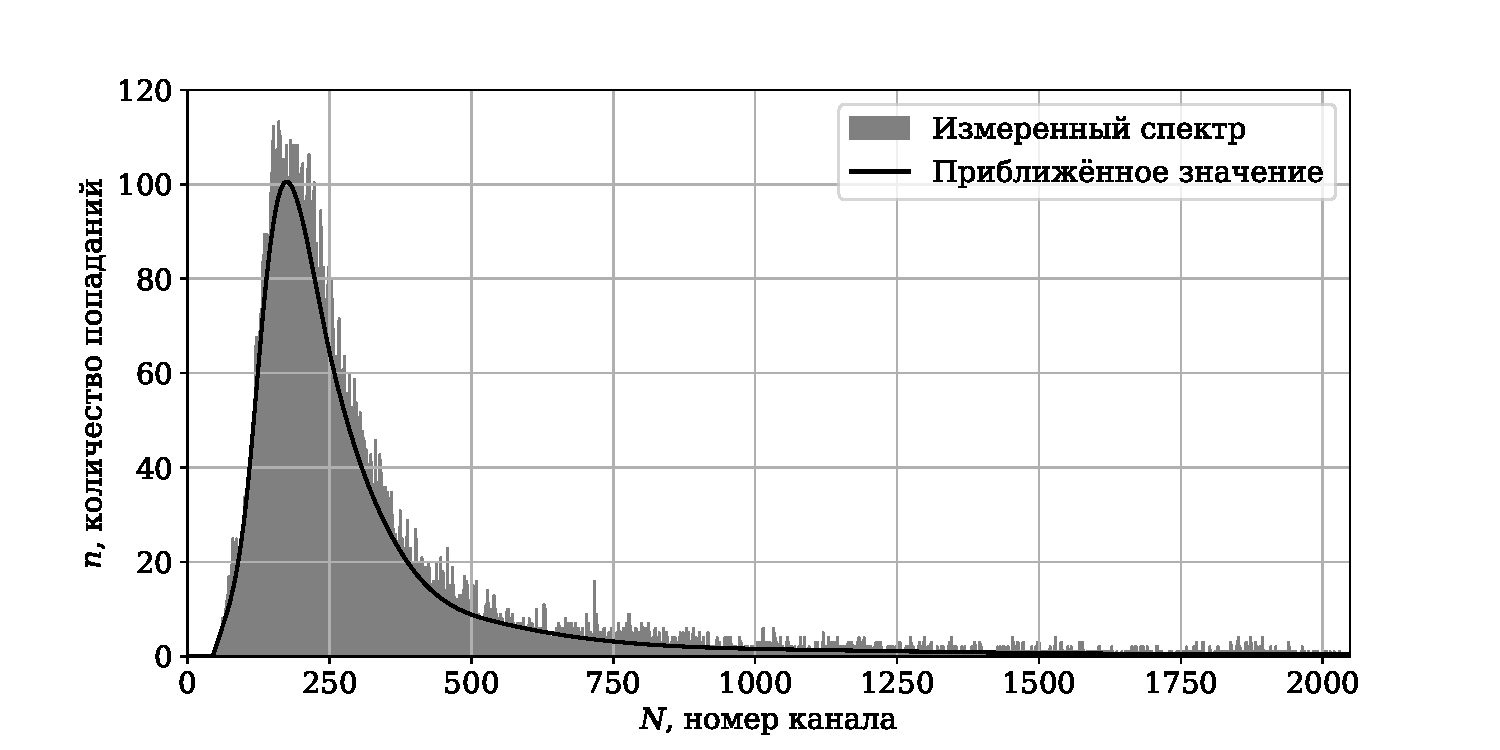
\includegraphics[width=\textwidth]{spectrum_bg.pdf}
\caption{Спектр фонового излучения}
\label{fig:bg}
\end{figure}

\subsection{Калибровка оси}

\paragraph{}По измеренным спектрам для $^{22}$Na, $^{60}$Co и $^{137}$Cs найдём положения известный гамма-линий и по измеренным данным построим калибровочную прямую. Для измерения положения гамма-линии будем приближать её гауссианом (\mintinline{python}|curve_fit| из scipy):

\begin{equation}
y = A \exp{\left( - \frac{(x - x_0)^2}{2 \sigma^2} \right)}.
\label{e:gauss}
\end{equation}

Полученные значения запишем в таблицу \ref{tab:calib}. По полученным данным построим калибровочную прямую (рис. \ref{fig:calib}). Полученной значение $\mathcal{E} = 0.797 \cdot N - 32$.

\begin{table}[h]
\centering
\begin{tabular}{|l|l|l|l|l|l|}
\hline
Полоса             & $^{22}$Na (1) & $^{22}$Na (2) & $^{60}$Co (1) & $^{60}$Co (2) & $^{137}$Cs \\ \hline
$\mathcal{E}$, кэВ & 1274          & 511           & 1332.5        & 1173.2        & 661.7      \\ \hline
$x_0$              & 1641          & 681.6         & 1716          & 1510          & 871.6      \\ \hline
$\Delta x_0$       & 3             & 0.7           & 1             & 1             & 0.4        \\ \hline
\end{tabular}
\caption{Данные для построения калибровочной прямой}
\label{tab:calib}
\end{table}

\begin{figure}[h]
\centering
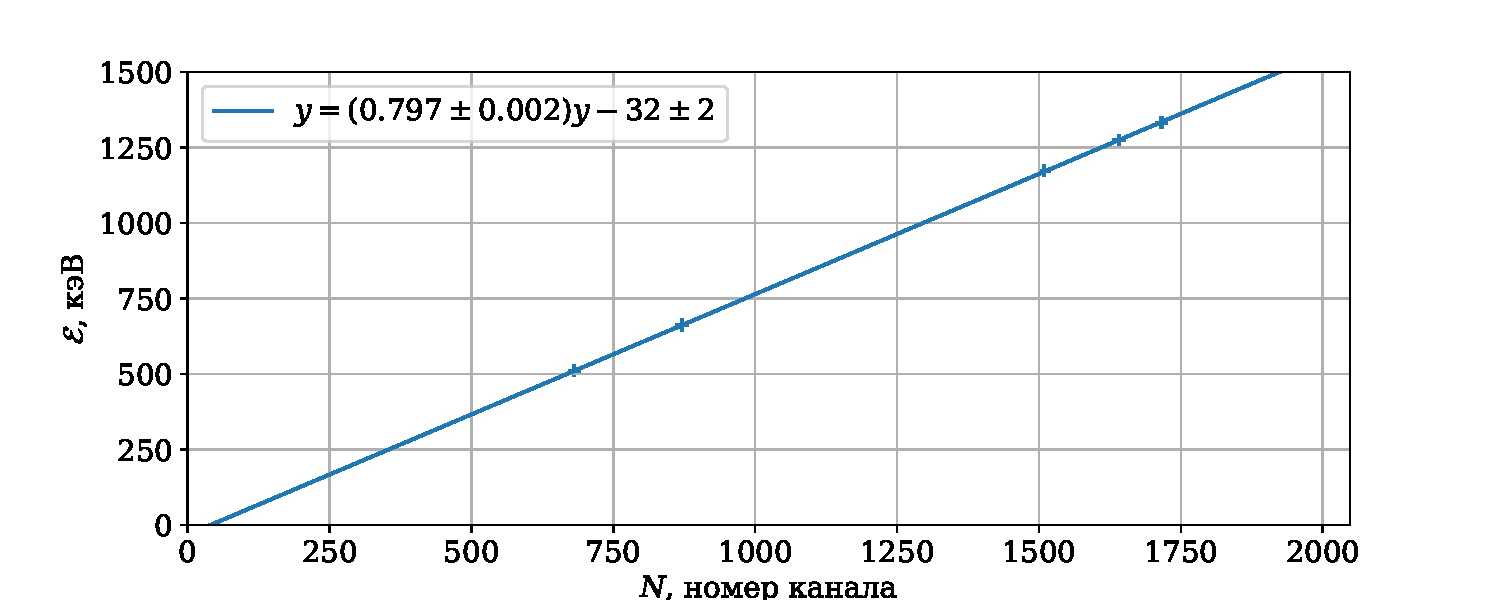
\includegraphics[width=\textwidth]{calibration.pdf}
\caption{График калибровочной прямой}
\label{fig:calib}
\end{figure}

\subsection{Анализ спектров}

\paragraph{}Используем калибровочную прямую для построения измеренных спектров в энергетических координатах (рис. \ref{fig:am}--\ref{fig:na}). Приближая пики гамма-линий гауссианами (\ref{e:gauss}) найдём их положение и ширину на полу-высоте, примерно равной двум среднеквадратичным отклонениям $2\sigma$ (табл. \ref{tab:peaks}). 

\paragraph{}Измерим энергии краёв комптоновского излучения (На рис. \ref{fig:am}--\ref{fig:na} обозначены буквой $K$). Рассчитаем теоретическое значение по формуле \eqref{e:compton}:

\begin{equation}
E_{\max} = K = \frac{\hbar \omega}{1 + \frac{m_e c^2}{2 \hbar \omega}} = \frac{\mathcal{E}_\gamma}{1 + \frac{511 \text{ кэВ}}{2 \mathcal{E}_\gamma}},
\end{equation}

\noindent построим график измеренных и рассчитанных значений (рис. \ref{fig:compton}). Видим, что значения получились очень похожими.

\paragraph{}По данным из таблицы \ref{tab:peaks} проверим соотношение \eqref{e:res_law}. Для этого построим график зависимости $R^2 = f(1/\mathcal{E})$ (рис. \ref{fig:resolution}). Видим, что разброс точек достаточно большой, но при этом некая зависимость наблюдается.

\paragraph{}Измерим энергии обратного рассеяния (На рис. \ref{fig:am}--\ref{fig:na} обозначены буквой $B$). Рассчитаем теоретическое значение по формуле \eqref{e:compron_back}:

\begin{equation}
E_{\max} = B = \frac{\mathcal{E}_\gamma}{1 + \frac{2 \mathcal{E}_\gamma}{511 \text{ кэВ}}},
\end{equation}

\noindent также построим график измеренных и рассчитанных значений (рис. \ref{fig:compton_back}). Видим, что значения похожи на теоретические.

\paragraph{} Учтём характеристическое излучение свинца. Энергии характеристического излучения соответствующие $K \alpha_1$,$K \alpha_2$ и $K \beta_1$ переходам соответственно равны $75, 73, 86$ кэВ. Однако на измеренных спектрах таких значений не наблюдается, из чего можно сделать вывод, что вклад характеристического излучения свинца в спектр незначителен.

\begin{table}[]
\centering
\begin{tabular}{|l|l|l|l|}
\hline
Источник        & $\mathcal{E}$, кэВ & $2 \sigma$, кэВ & $R$  \\ \hline
$^{241}$Am      & 67                 & 14              & 0.21 \\ \hline
$^{152}$Eu$(1)$ & 43                 & 16              & 0.37 \\ \hline
$^{152}$Eu$(2)$ & 129                & 18              & 0.14 \\ \hline
$^{152}$Eu$(3)$ & 245                & 38              & 0.16 \\ \hline
$^{152}$Eu$(4)$ & 345                & 36              & 0.10 \\ \hline
$^{152}$Eu$(5)$ & 777                & 88              & 0.11 \\ \hline
$^{152}$Eu$(6)$ & 960                & 92              & 0.10 \\ \hline
$^{152}$Eu$(7)$ & 1105               & 90              & 0.08 \\ \hline
$^{152}$Eu$(8)$ & 1414               & 80              & 0.06 \\ \hline
$^{137}$Cs$(0)$ & 32                 & 18              & 0.56 \\ \hline
$^{137}$Cs$(1)$ & 662                & 48              & 0.07 \\ \hline
$^{60}$Co$(1)$  & 1170               & 78              & 0.07 \\ \hline
$^{60}$Co$(2)$  & 1335               & 74              & 0.06 \\ \hline
$^{22}$Na$(1)$  & 511                & 42              & 0.08 \\ \hline
$^{22}$Na$(2)$  & 1275               & 76              & 0.06 \\ \hline
\end{tabular}
\caption{Пики полного поглощения на измеренных спектрах}
\label{tab:peaks}
\end{table}

\begin{figure}
\centering
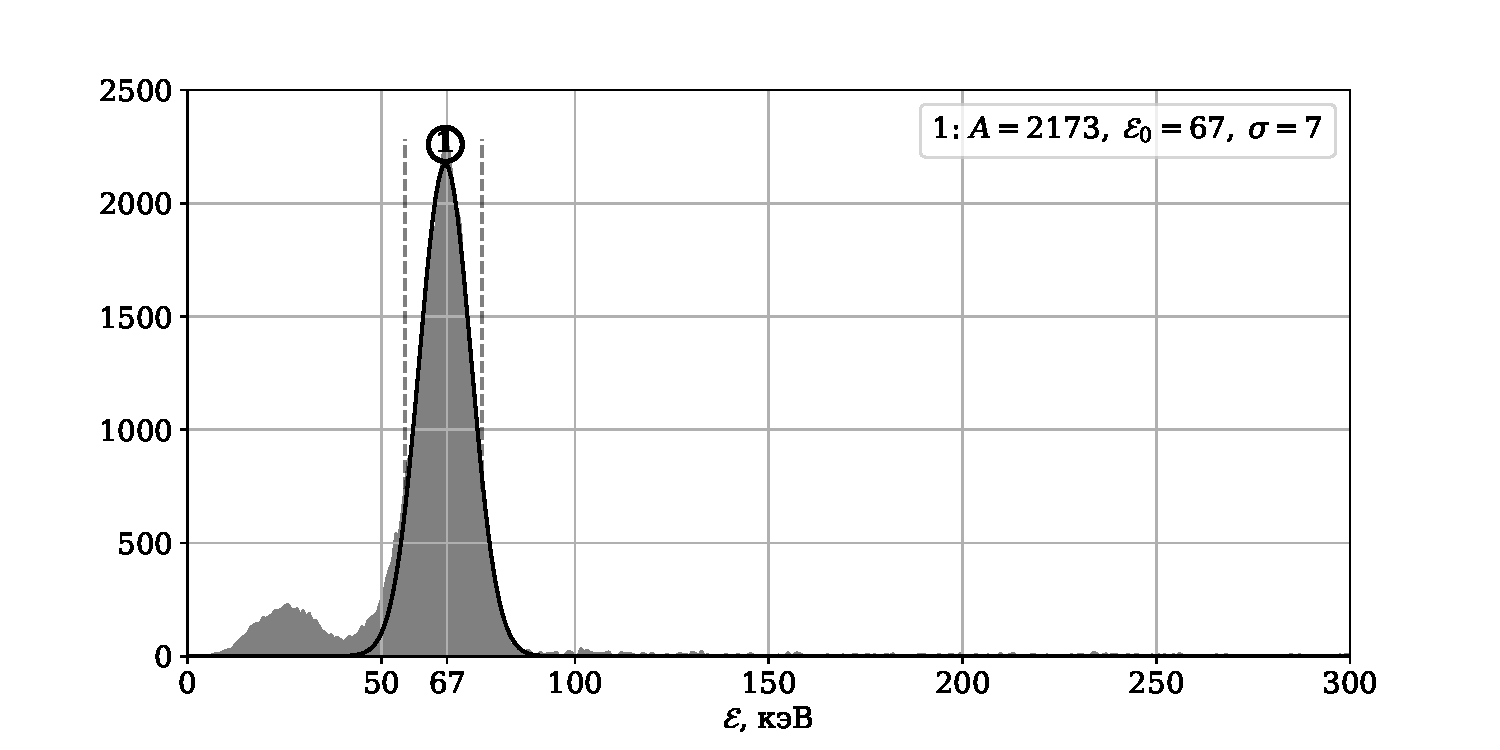
\includegraphics[width=\textwidth]{spectrum_am.pdf}
\caption{Спектр $^{241}_{95}$Am}
\label{fig:am}
\end{figure}

\begin{figure}
\centering
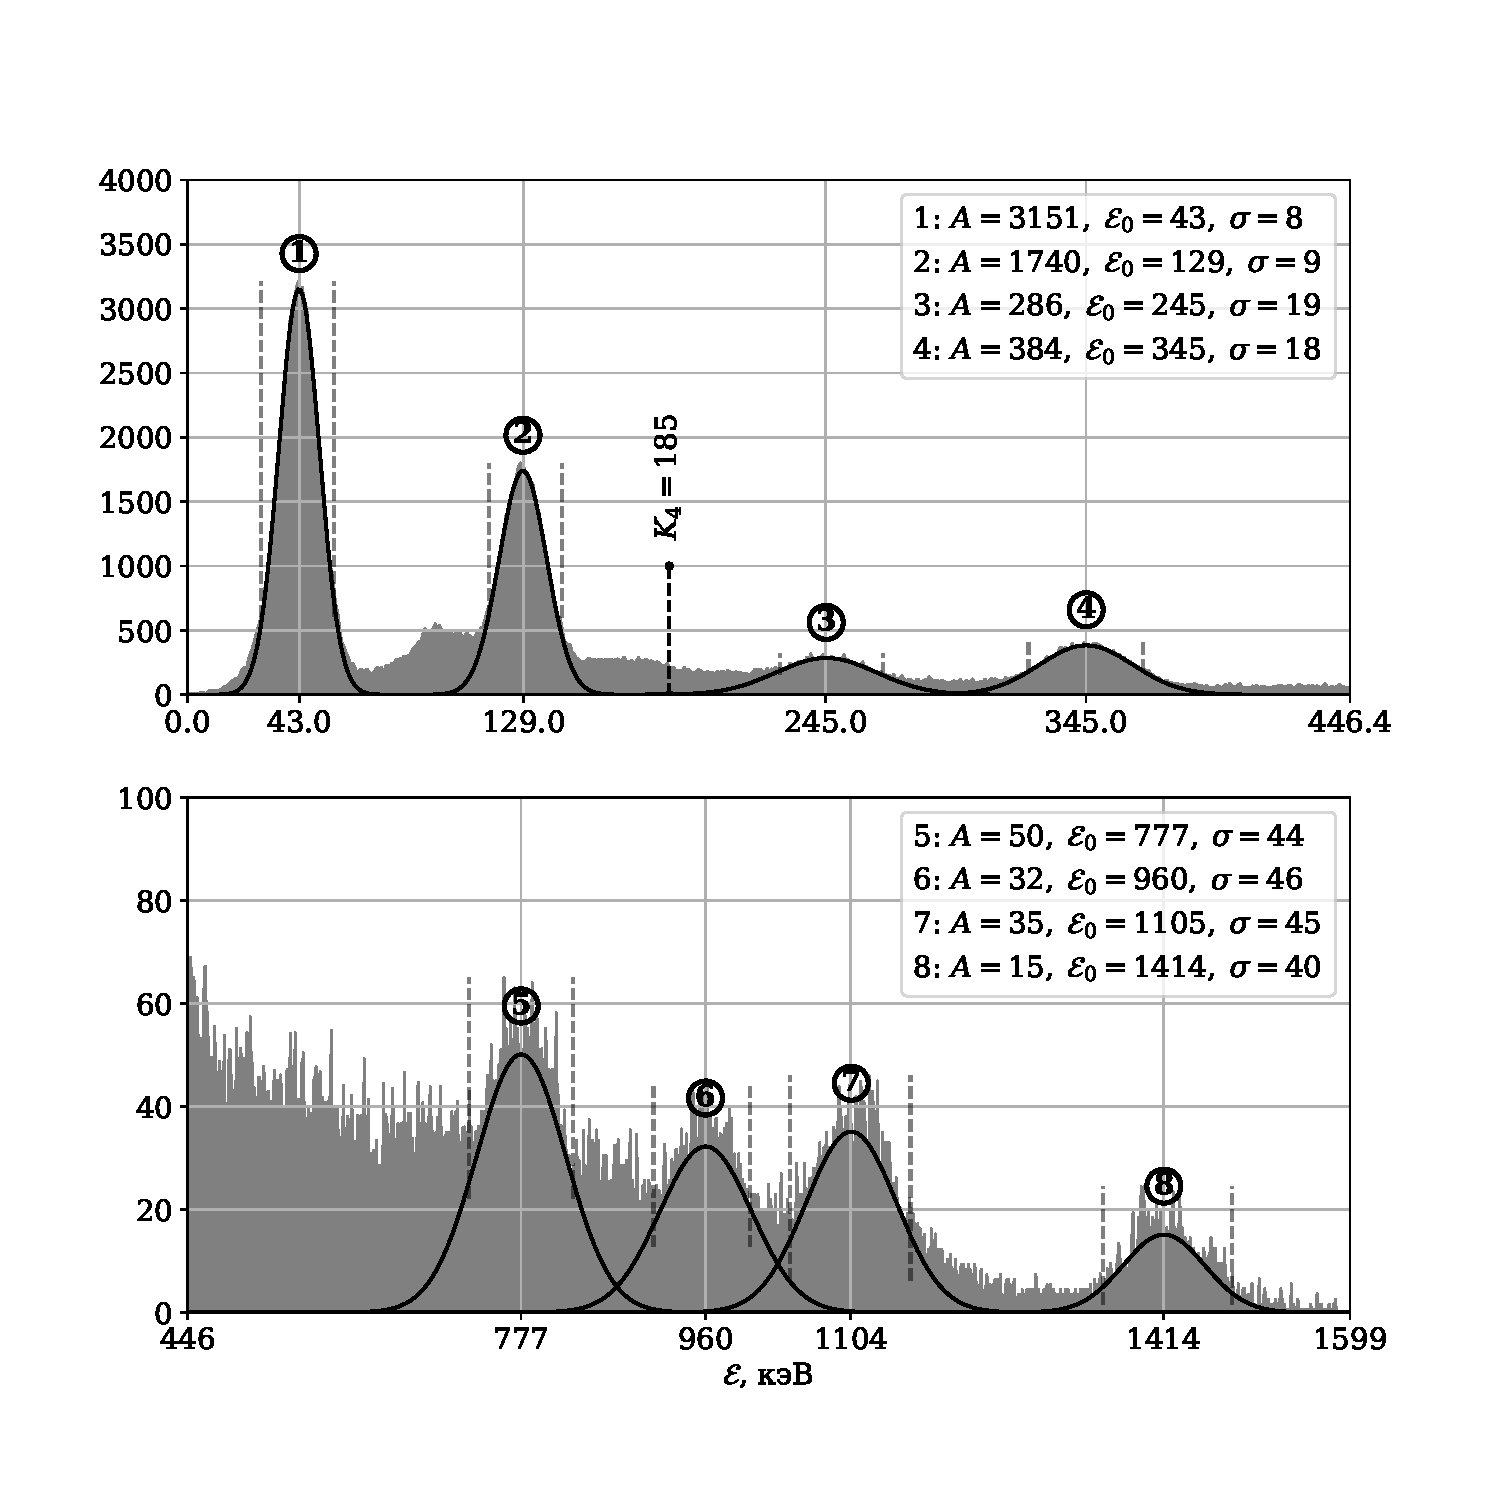
\includegraphics[width=\textwidth]{spectrum_eu.pdf}
\caption{Спектр $^{152}_{63}$Eu}
\label{fig:eu}
\end{figure}

\begin{figure}
\centering
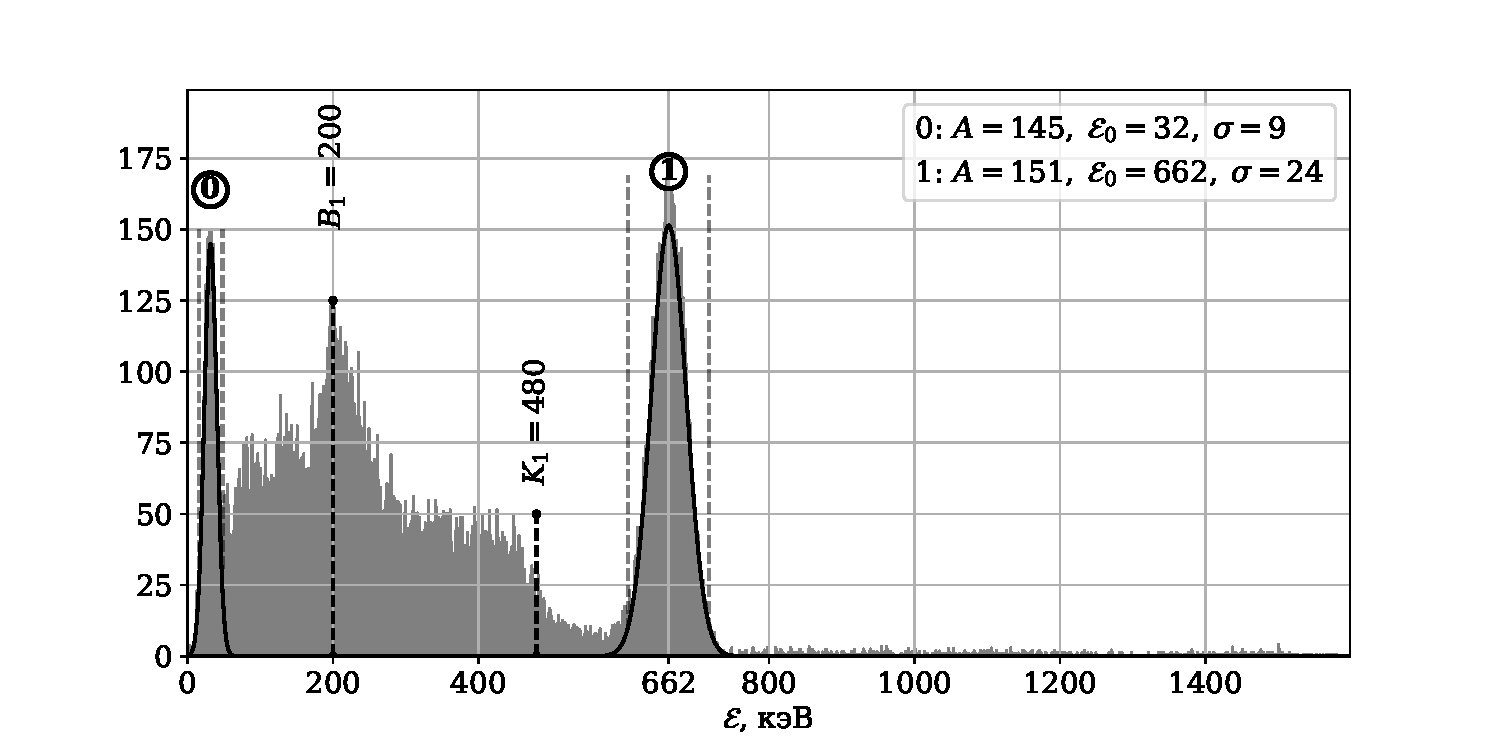
\includegraphics[width=\textwidth]{spectrum_cs.pdf}
\caption{Спектр $^{137}_{55}$Cs}
\label{fig:cs}
\end{figure}

\begin{figure}
\centering
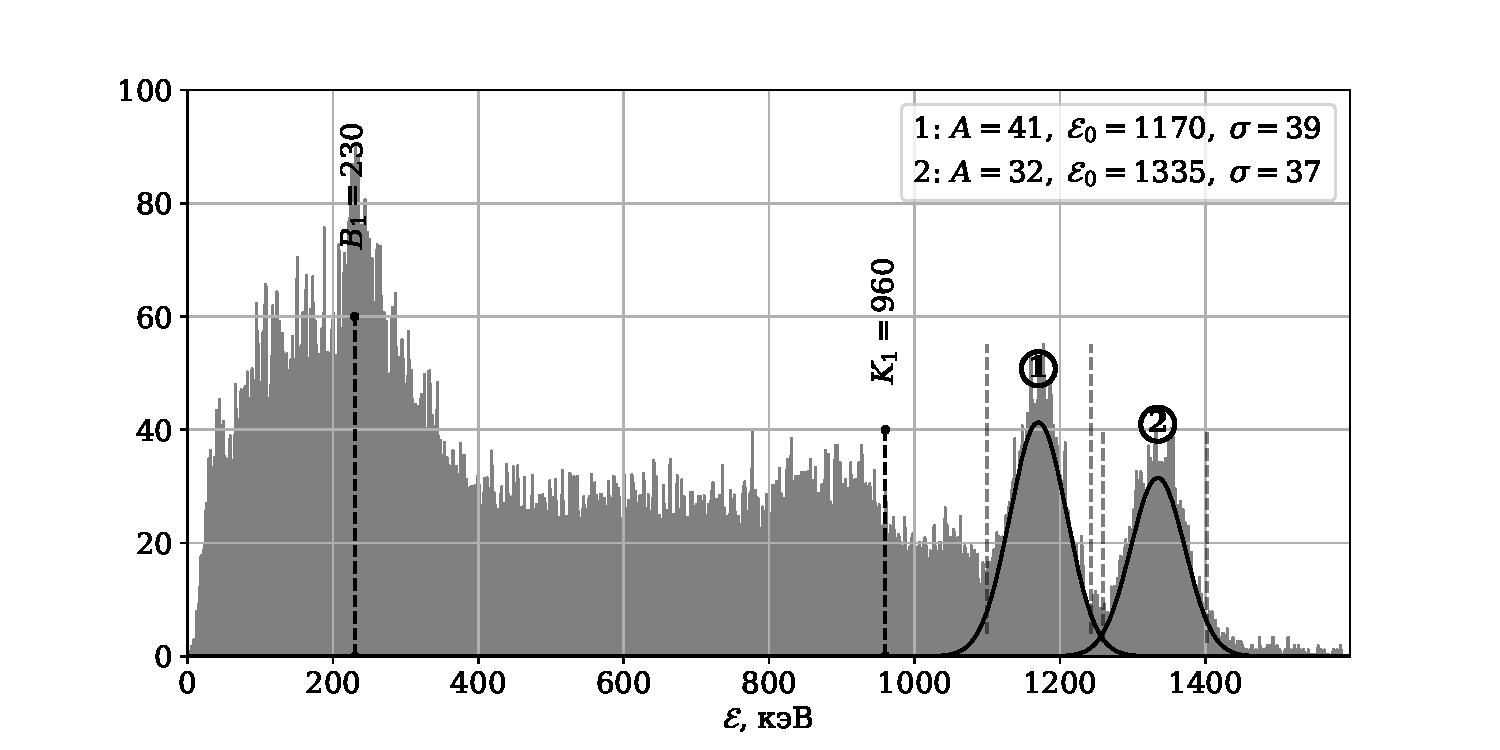
\includegraphics[width=\textwidth]{spectrum_co.pdf}
\caption{Спектр $^{60}_{27}$Co}
\label{fig:co}
\end{figure}

\begin{figure}
\centering
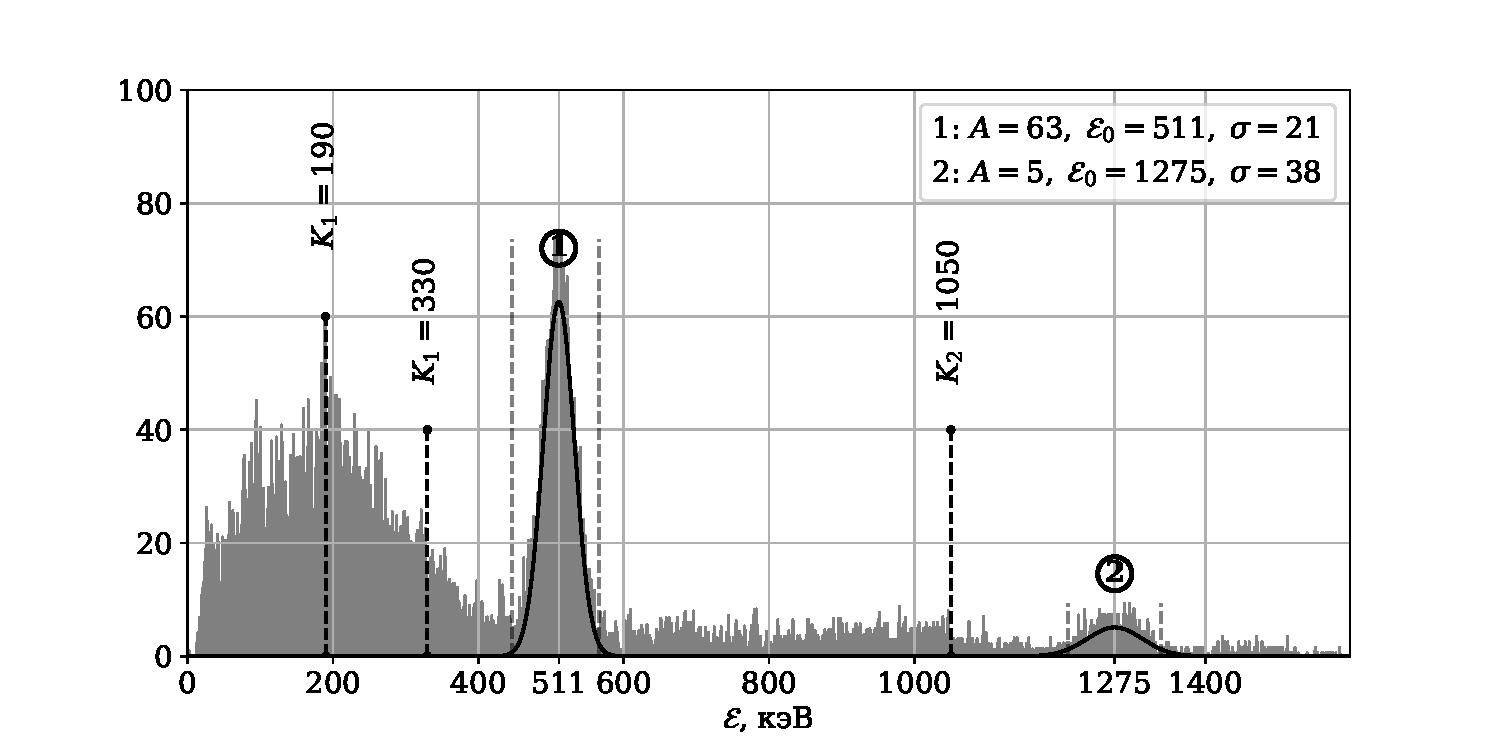
\includegraphics[width=\textwidth]{spectrum_na.pdf}
\caption{Спектр $^{22}_{11}$Na}
\label{fig:na}
\end{figure}

\begin{figure}
\centering
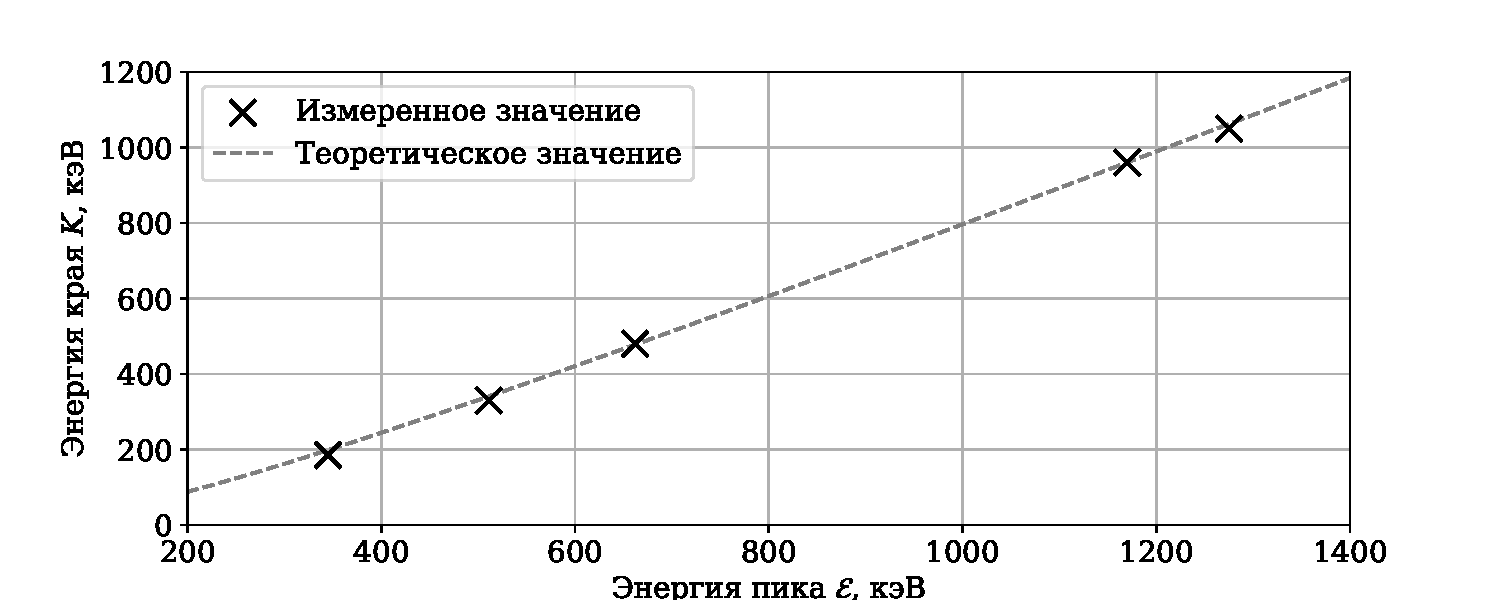
\includegraphics[width=\textwidth]{compton.pdf}
\caption{\centering График рассчитанных и измеренных значений энергий краёв комптоновского спектра}
\label{fig:compton}
\end{figure}

\begin{figure}
\centering
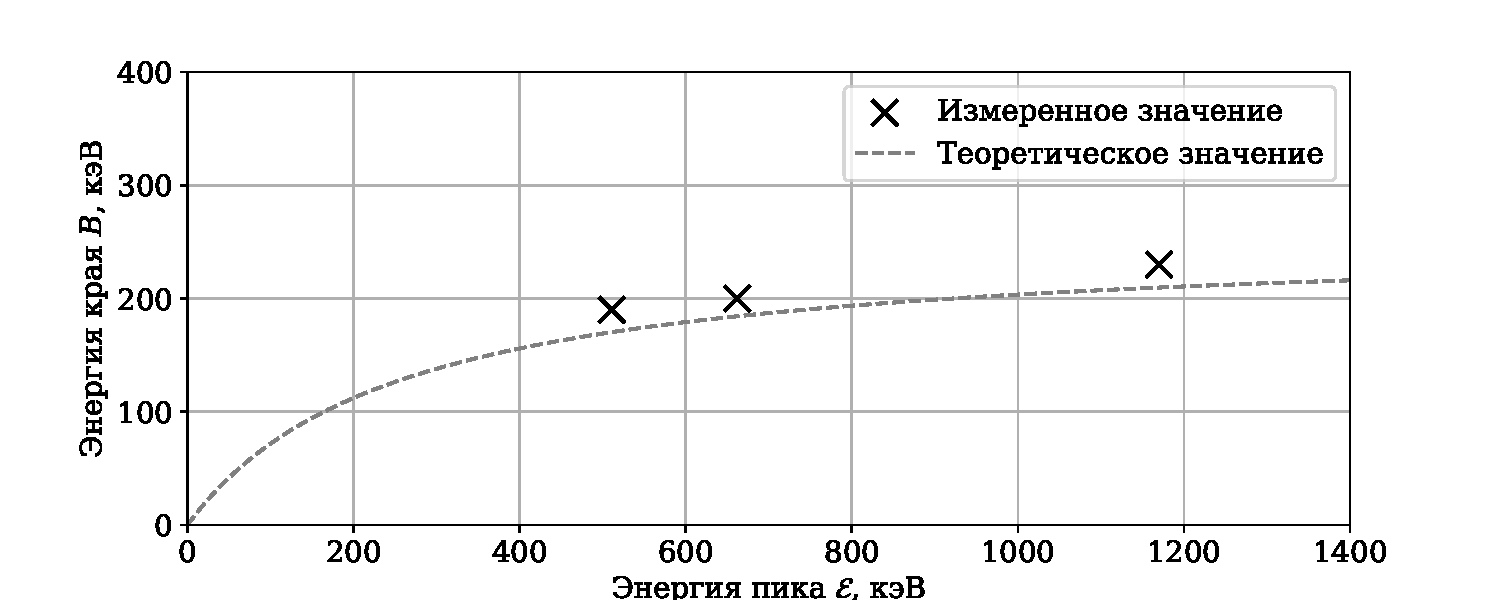
\includegraphics[width=\textwidth]{compton_back.pdf}
\caption{\centering График рассчитанных и измеренных значений энергий обратного рассеяния}
\label{fig:compton_back}
\end{figure}

\begin{figure}
\centering
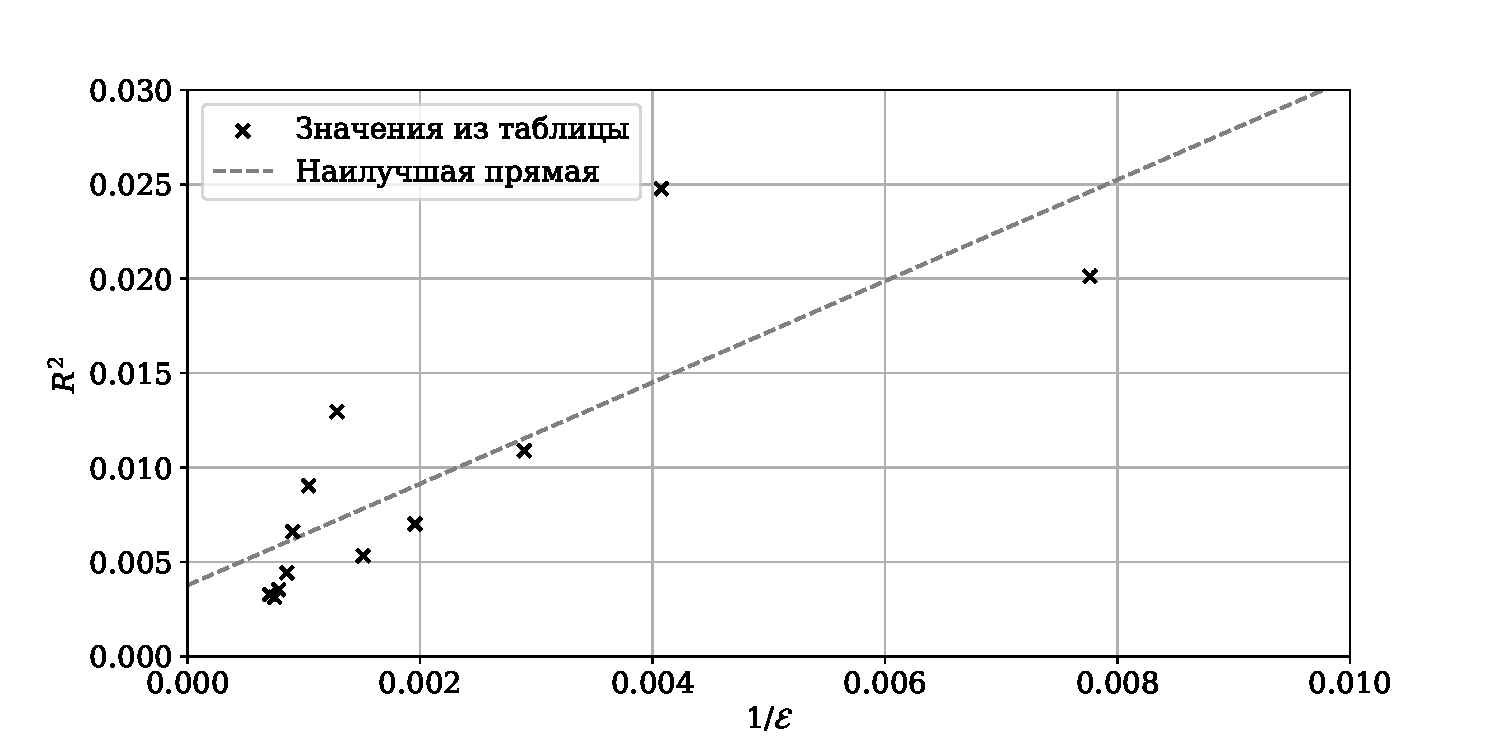
\includegraphics[width=\textwidth]{resolution.pdf}
\caption{График зависимости $R^2 = f(1/\mathcal{E})$ }
\label{fig:resolution}
\end{figure}

\medskip\hrule\medskip

\section{Выводы}

\begin{enumerate}
\item Изучили работу сцинтилляционного гамма-спектрометра, получив гамма-спектры для образцов.
\item По известным спектральным линиям откалибровали спектры по энергии.
\item Определили положения гамма-линий для остальных образцов.
\item Проверили эффект Комптона, сравнив измеренные энергии верхнего и нижнего край комптоновского рассеяния с теоретическими.
\item Проверили зависимость ширины спектральной линии от энергии линии.
\end{enumerate}

\medskip\hrule\medskip

\end{document}
